\section{Notation and Terminology}
\label{sec:prelims}

% Initially taken from Kyle's dissertation.

% Temporary definition to allow compilation of lazily copied prelim section:

\note{Jeff: Revisit after the rest of the paper is finished.}

We begin by recalling several useful definitions related to surface-embedded graphs.  For further background, we refer the reader to Gross and Tucker \cite{gt-tgt-01} or Mohar and Thomassen~\cite{mt-gs-01} for topological graph theory, and to Hatcher~\cite{h-at-02} or Stillwell~\cite{s-ctcgt-93} for surface topology and homology.


\note{Erin and Kyle: Assume uniqueness of shortest paths somewhere in the prelims!  Cite appropriate stuff.}

\subsection{Surfaces and curves}

A \EMPH{surface} (more formally, a \emph{2-manifold with boundary}) is a compact Hausdorff space in which every point has an open neighborhood homeomorphic to either the plane $\Real^2$ or a closed halfplane $\set{(x,y)\in \Real^2\mid x\ge 0}$.  The points with halfplane neighborhoods make up the \EMPH{boundary} of the surface; every component of the boundary is homeomorphic to a circle.
A surface is \EMPH{non-orientable} if it contains a subset homeomorphic to
the M\"obius band, and \EMPH{orientable} otherwise. In this paper, we consider only compact, connected, and orientable surfaces.
\note{Kyle: I guess we can do non-orientable, at least for computing minimal directed cycles, although the Betti numbers get nastier.}

A \EMPH{path} in a surface $\Sigma$ is a continuous function $p\colon [0,1]\to\Sigma$.
A \EMPH{loop} is a path whose endpoints~$p(0)$ and~$p(1)$ coincide;
we refer to this common endpoint as the \EMPH{basepoint} of the loop.
An \EMPH{arc} is a path internally disjoint from the boundary of~$\Sigma$
whose endpoints lie on the boundary of $\Sigma$.
A \EMPH{cycle} is a continuous function $\gamma\colon S^1\to\Sigma$;
the only difference between a cycle and a loop is that a loop has a
distinguished basepoint.
We say a loop~$\ell$ and a cycle~$\gamma$ are \EMPH{equivalent} if, for some
real number~$\delta$, we have~$\ell(t) = \gamma(t + \delta)$ for
all~$t \in [0,1]$.
We collectively refer to paths, loops, arcs, and cycles as \EMPH{curves}.
A curve is \EMPH{simple} if it is injective; we usually do not distinguish between simple curves and their images in $\Sigma$.
A simple curve~$p$ is \EMPH{separating} if~$\Sigma \setminus p$ is disconnected.

The \EMPH{reversal}~$\rev(p)$ of a path~$p$ is defined by
setting~$\rev(p)(t) = p(1-t)$. The \EMPH{concatenation}~$p \cdot q$ of two
paths~$p$ and~$q$ with~$p(1)=q(0)$ is the path created by
setting~$(p\cdot q)(t) = p(2t)$ for all~$t \leq 1/2$
and~$(p\cdot q)(t) = q(2t-1)$ for all~$t \geq 1/2$.
% Kyle: I removed the definition for subpath p[x,y], because I don't think we use it.

The \EMPH{genus} of a surface $\Sigma$ is the maximum number of disjoint simple cycles in $\Sigma$ whose complement is connected.
 Up to homeomorphism,
there is exactly one orientable surface and one non-orientable surface with any genus $g\ge 0$ and any number of
boundary cycles $b\ge 0$.
Orientable surfaces with~$b$ boundary components are differentiated by their \EMPH{Euler characteristic} ${\chi = 2 - 2g - b}$ (for non-orientable surfaces, ${\chi = 2 - g - b}$).


\subsection{Graph embeddings}

An \EMPH{embedding} of an undirected graph $G=(V,E)$ on a surface $\Sigma$ maps vertices to distinct points and edges to simple, interior-disjoint paths.  The \EMPH{faces} of the embedding are maximal connected subsets of $\Sigma$ that are disjoint from the image of the graph.
We may denote an edge~$uv \in E$ as~$f | g$ if it is incident to faces~$f$ and~$g$.
An embedding is \EMPH{cellular} if each of its faces is homeomorphic to the plane; in particular, in any cellular embedding, each component of the boundary of $\Sigma$ must be covered by a cycle of edges in $G$.  Euler's formula implies that any cellularly embedded graph with $n$ vertices, $m$ edges, and $f$ faces lies on a surface with Euler characteristic $\chi = n-m+f$, which implies that $m = O(n+g)$ and $f=O(n+g)$
if the graph is simple.
We consider only such
cellular embeddings of genus $g=O(n^{1-\eps})$, so that the overall complexity of the embedding is $O(n)$.

Any cellular embedding on an orientable surface can be encoded combinatorially
by a \EMPH{rotation system}, which records the counterclockwise order of edges
incident to each vertex.
Two paths or cycles in a combinatorial surface \EMPH{cross} if no continuous infinitesimal perturbation makes them disjoint; if such a perturbation exists, then the paths are \EMPH{non-crossing}.

We redundantly use the term \EMPH{arc} to refer to a walk in the graph whose endpoints are boundary vertices.  Likewise, we use the term \EMPH{cycle} to refer to a closed walk in the graph. 
Note that cycles may contain the same vertex or edge more than once.

\begin{figure}[t]
\centering
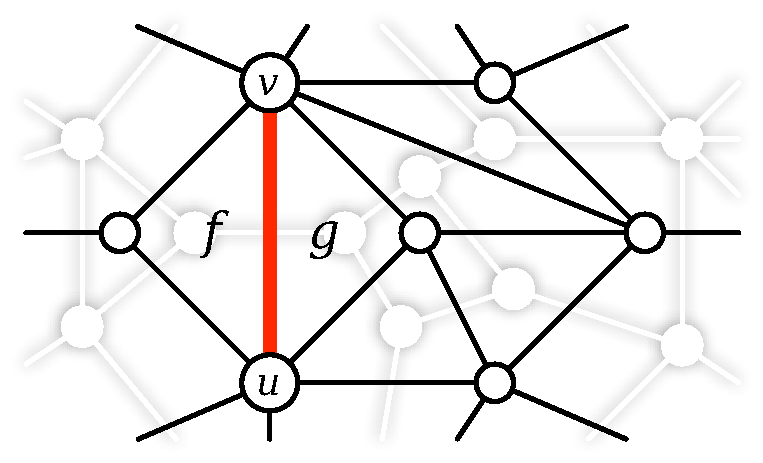
\includegraphics[height=0.9in]{Fig/primal}\quad
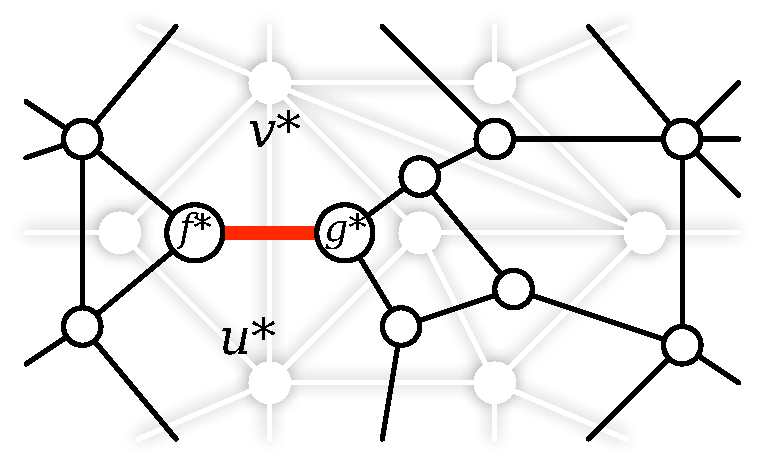
\includegraphics[height=0.9in]{Fig/dual}
\caption{Graph duality.  One edge $uv$ and its dual $(uv)^* =
f^*g^*$ are emphasized.} \label{fig:prelims_primaldual}
\end{figure}

Any undirected graph~$G$ embedded on a surface~$\Sigma$ without boundary has a
\EMPH{dual graph}~$G^*$, which has a vertex~$f^*$ for each face~$f$ of~$G$,
and an edge~$e^*$ for each edge~$e$ in~$G$ joining the vertices dual to the
faces of~$G$ that~$e$ separates. The dual graph~$G^*$ has a natural cellular
embedding in~$\Sigma$, whose faces corresponds to the vertices of~$G$.
See Figure~\ref{fig:prelims_primaldual}.
For any subgraph~${F = (U, D)}$ of~$G=(V,E)$, we write~$G \setminus F$
to denote the edge-complement~$(V,E \setminus D)$. We also abuse notation
by writing~$F^*$ to denote the subgraph of~$G^*$ corresponding to any
subgraph~$F$ of~$G$.
Further, we may sometimes use~$D$ to refer to an edge set or the subgraph~$F = (V, D)$,
but it should be clear which we mean from context.

For the problem we consider in Section~\ref{sec:homcover}, the input is actually a \emph{directed} edge-weighted
graph~$G$ with a cellular embedding on some surface.
We use the
notation~$u \arcto v$ to denote the directed \EMPH{dart} from vertex~$u$ to vertex~$v$, and let~$\vec{E}$ be the set of darts in~$G$.
Without loss of generality, we consider only \EMPH{symmetric} directed graphs,
in which the reversal~$v \arcto u$ of any dart~$u \arcto v$ is another dart,
possibly with weight~$0$.
We also assume that in the cellular embedding,
the images of any edge in~$G$ and its reversal coincide (but with opposite
orientations).
The two darts~$u \arcto v$ and~$v \arcto u$ therefore define an \EMPH{edge}~$uv$
with a canonical orientation~$u \arcto v$; edge~$vu$ does not necessarily exist even though~$uv$ does.
Thus, like other authors~\cite{ccl-fsncd-10,e-sncds-11,f-sntcd-13},
we implicitly model directed graphs as \emph{undirected graphs with asymmetric
edge weights}.
The dual of any dart with face~$f$ to its left and~$g$ to its right is~$f^* \arcto g^*$.
Note that the duality of darts is \emph{not} an involution the way we have specified the orientation of the dual dart here.

\subsection{Homotopy and homology}

Two paths~$p$ and~$q$ in $\Sigma$ are \EMPH{homotopic} if one can be
continuously deformed into the other without changing their endpoints.
More formally, a \EMPH{homotopy} between~$p$ and~$q$ is a
continuous map $h\colon {[0,1]\times [0,1] \to \Sigma}$ such that $h(0,\cdot) = p$, $h(1,\cdot) = q$, $h(\cdot, 0)=p(0)=q(0)$, and $h(\cdot,1)=p(1)=q(1)$.
Homotopy defines an equivalence relation over the set of paths with any
fixed pair of endpoints. The set of homotopy classes of loops in~$\Sigma$
with basepoint~$x_0$ defines a group~$\pi_i(\Sigma,x_0)$ under concatenation,
called the \EMPH{fundamental group} of~$\Sigma$. (For all basepoints~$x_0$
and~$x_1$, the groups~$\pi_i(\Sigma,x_0)$ and~$\pi_i(\Sigma,x_1)$ are
isomorphic.) A cycle is \EMPH{contractible} if it is homotopic to a constant
map.
Given a weight function on the darts of~$G$, we say a directed path or cycle is \EMPH{tight} if it has minimum total weight (counting edges with multiplicity) for its homotopy class.

Homology is a coarser equivalence relation than homotopy, with nicer
algebraic properties.  Like several earlier papers \cite{cf-qhc2-07,
cf-qhc-08, dls-chtl-07, dlsc-cgaht-08,e-sncds-11,f-sntcd-13}, we will consider only
one-dimensional cellular homology with coefficients in the finite
field $\Z_2$; this restriction allows us to radically simplify our
definitions.
Fix a cellular embedding of an undirected graph $G$ on a surface with genus $g$ and $b$ boundaries.  An \EMPH{even subgraph} is a subgraph of $G$ in which every node has even degree, or equivalently, the union of edge-disjoint cycles.  A \EMPH{boundary subgraph} is the boundary of the union of a subset of faces of $G$; for example, every separating cycle is a boundary subgraph.

Two even subgraphs are \EMPH{homologous}, or in the same \EMPH{homology class}, if their symmetric difference is a boundary subgraph.
Boundary subgraphs are also called \EMPH{null-homologous}.  Any two homotopic cycles are homologous, but homologous cycles are not necessarily homotopic; see Figure \ref{F:homology}.  Moreover, the homology class of a cycle can contain even subgraphs that are not cycles; see Figure \ref{F:homology2}.

\note{Erin: No mention of Betti number, but we do use it later.  Add here?}

\begin{figure}[htb]
\centering
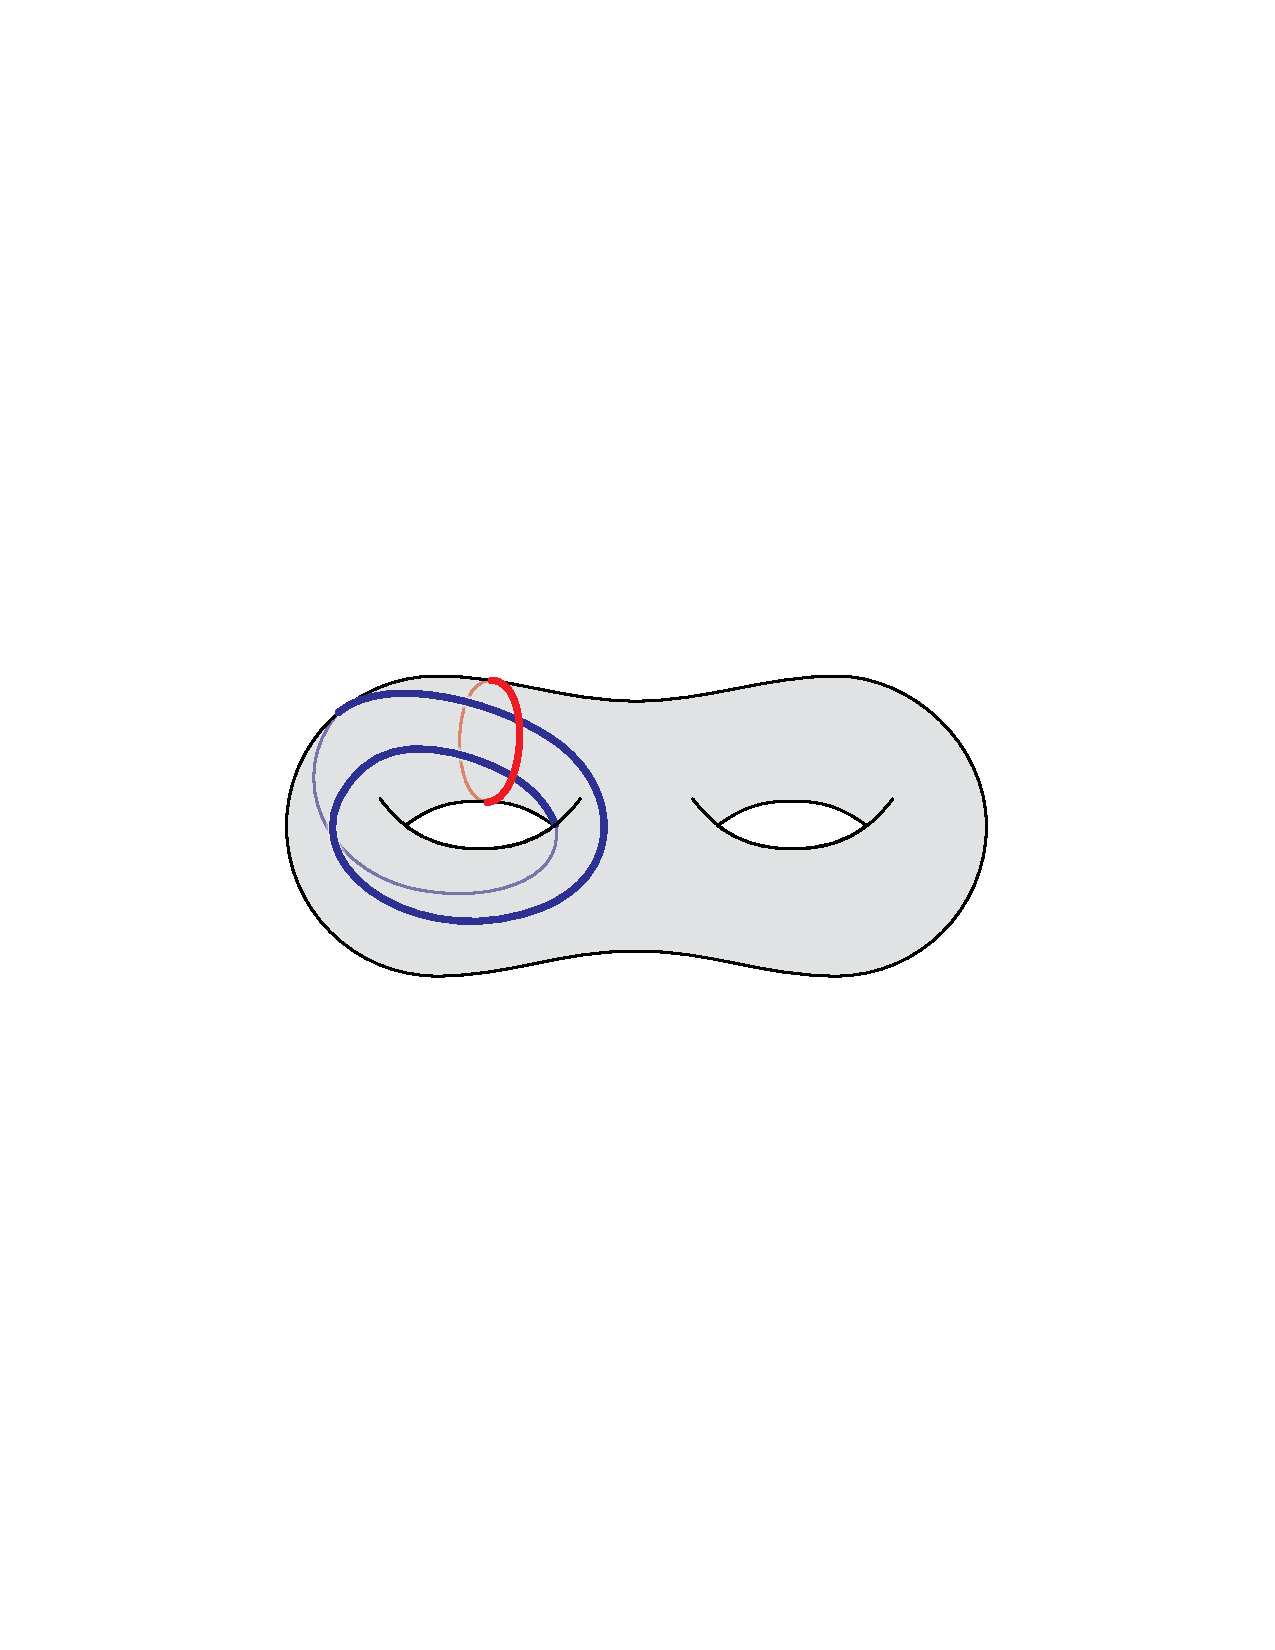
\includegraphics[height=0.75in]{Fig/homologous3}\\[2ex]
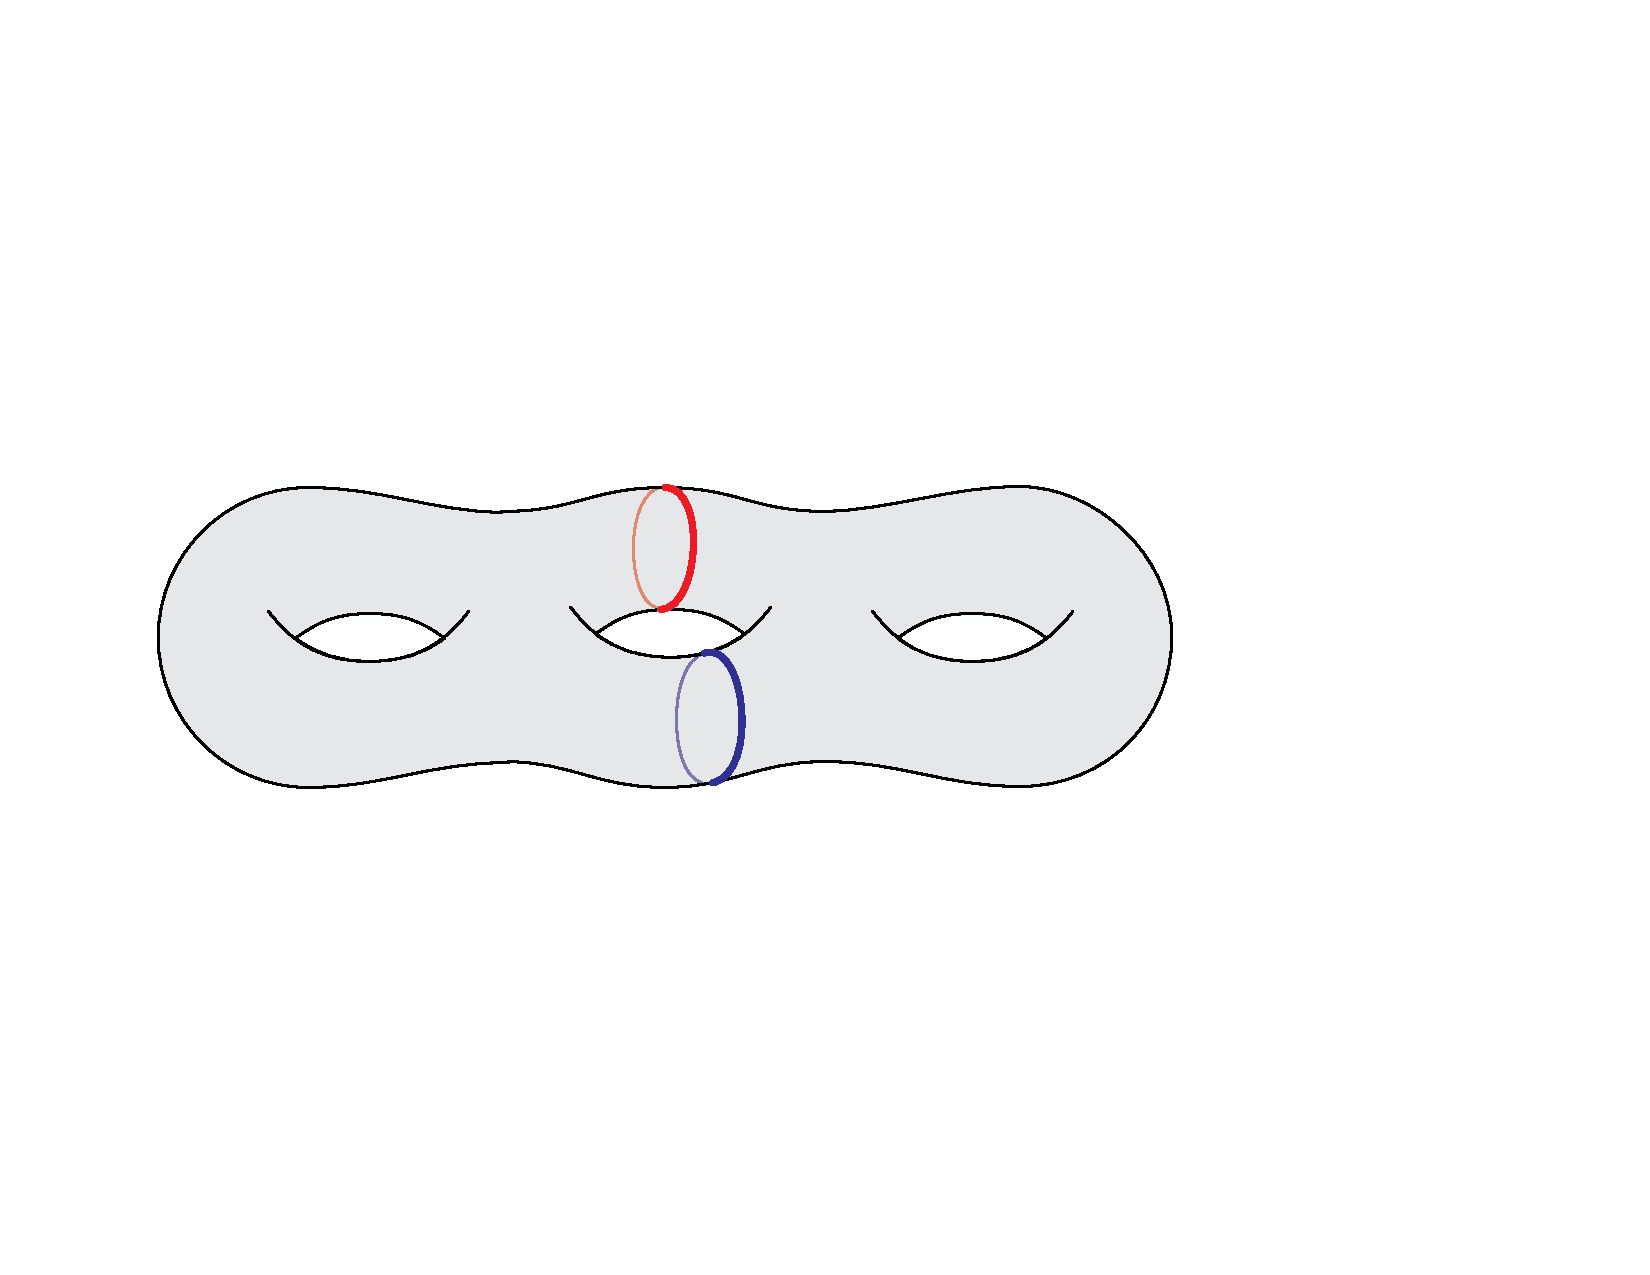
\includegraphics[height=0.75in]{Fig/homologous2}
\caption{Homologous pairs of cycles that are not homotopic.  (Lighter portions of the curves are on the back side of the surface.)}
\label{F:homology}
\end{figure}

\begin{figure}[htb]
\centering
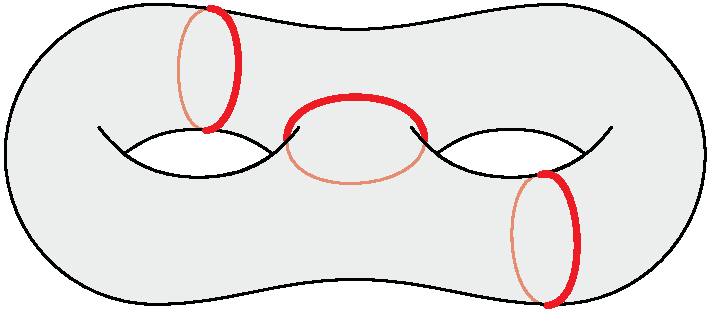
\includegraphics[height=0.75in]{Fig/homologous1}
\caption{Each cycle is homologous to the union of the other two.}
\label{F:homology2}
\end{figure}

\subsection{Cut-even subgraph duality}
\note{Kyle: The lemma below is key to the algorithms working, but there doesn't appear to be enough there to make them their own section. Where should we put them?}

\note{Erin: I don't like it in the prelims, since it is not previous work.  One thought: perhaps the beginning of section 4, as a new subsection?  Then we can cite it in 4.2 as why this solves the min cut problem.}

A crucial component of our minimum $(s,t)$-cut algorithms is an equivalence between $(s,t)$-cuts and even subgraphs of the \emph{dual graph} contained in a particular homology class.
We formalize this equivalence in the following lemma.

\begin{lemma}
\label{lem:cut-duality}
Let $G$ be an edge-weighted graph embedded on a surface $\Sigma$ without boundary, and let $s$ and $t$ be vertices of~$G$.  Finally, let $C$ be the minimum-weight $(s,t)$-cut in~$G$.  Then~$C^*$ is the minimum-weight even subgraph of $G^*$ homologous with the boundary of $s^*$ in the surface $\Sigma\setminus(s^*\cup t^*)$.
\end{lemma}

\begin{proof}
Let $\partial s^*$ denote the boundary of $s^*$, and let $\Sigma'$ denote the surface $\Sigma\setminus {(s^*\cup t^*)}$.

Let $C$ be an arbitrary $(s,t)$-cut in $G$.  This cut partitions the vertices of $G$ into two disjoint subsets, $S$ and $T$, respectively containing vertices $s$ and $t$.  Thus, the dual subgraph $C^*$ partitions the faces of $G^*$ into two disjoint subsets, $S^*$ and $T^*$, respectively containing faces $s^*$ and $t^*$.  In particular, $C^*$ is the boundary of the union of the faces in $S^*$, which implies that $C^*$ is null-homologous in $\Sigma$.  The subgraph $C^* \oplus \partial s^*$ is the boundary of the union of $S^* \setminus\set{s^*}$, which is a subset of the faces of $\Sigma'$.  Thus,  $C^*\oplus \partial s^*$ is null-homologous in $\Sigma'$.  We conclude that $C^*$ and  $\partial s^*$ are homologous in $\Sigma'$.

Conversely, let $C^*$ be an arbitrary even subgraph of $G^*$ homologous to $\partial s^*$ in $\Sigma'$.  The subgraph $C^*\oplus \partial s^*$ is null-homologous in $\Sigma'$.  This immediately implies that $C^*$ is null-homologous in $\Sigma$; moreover, faces $s^*$ and $t^*$ are on opposite sides of $C^*$.   any path from $s$ to $t$ in the original graph $G$ must traverse at least one edge of $C$.  We conclude that $C$ is an $(s,t)$-cut.
\end{proof}


\subsection{Covering spaces and cutting}

A continuous map~$\pi : \Sigma' \to \Sigma$ between two surfaces is called a
\EMPH{covering map} if each point~$x \in \Sigma$ lies in an open
neighborhood~$U$ such that (1)~$\pi^{-1}(U)$ is a countable union of disjoint
open sets~$U_1 \cup U_2 \cup \cdots$ and (2) for each~$i$, the
restriction~$\pi |_{U_i} : U_i \to U$ is a homeomorphism. If there is a covering
map~$\pi$ from~$\Sigma'$ to~$\Sigma$, we call~$\Sigma'$ a \EMPH{covering space}
of~$\Sigma$. The \EMPH{universal cover}~$\tilde{\Sigma}$ is the unique
simply-connected covering space of~$\Sigma$ (up to homeomorphism).
The universal cover is so named because it covers every path-connected
covering space of~$\Sigma$.

For any path~$p : [0,1] \to \Sigma$ such that~$\pi(x') = p(0)$ for some
point~$x' \in \Sigma'$, there is a unique path~$p'$ in~$\Sigma'$, called
a \EMPH{lift} of~$p$, such that~$p'(0) = x'$ and~$\pi \circ p' = p$. We also
say that~$p$ \EMPH{lifts} to~$p'$. Conversely, for any path~$p'$ in~$\Sigma'$,
the path~$\pi \circ p'$ is called a \EMPH{projection} of~$p'$.

We define a lift of a cycle~$\gamma : S^1 \to \Sigma$ to be the infinite
path~$\gamma' : \R \to \Sigma'$ such that
${\pi(\gamma'(t)) = \gamma(t \mod 1)}$
for all real~$t$. We call the path obtained by restricting~$\gamma'$ to any
unit interval a \EMPH{single-period lift} of~$\gamma$; equivalently, a
single-period lift of~$\gamma$ is a lift of any loop equivalent to~$\gamma$.
We informally say that a cycle is the~\EMPH{projection} of any of its
single-period lifts.

\EMPH{Cutting} a combinatorial surface along a cycle or  arc modifies both the surface and the embedded graph.
For any combinatorial surface $S = (\Sigma, G)$ and any simple cycle or arc $\gamma$ in~$G$, we define a new combinatorial surface \EMPH{$S \snip \gamma$} by taking the topological closure of $\Sigma \backslash \gamma$ as the new underlying surface; the new embedded graph contains two copies of each vertex and edge of $\gamma$, each bordering a new boundary.
Similar to covering spaces, we define the~\EMPH{projection} of a curve in~$S \snip \gamma$ as the natural mapping of points (or vertices and edges) to~$S$.
